% TeX root = ../../paper.tex

\section{Background}\label{sec:background}

We assume that the reader is familiar with the basic concept of a petri net. Nevertheless, we quickly introduce the fundamentals in this chapter. In addition, the \emph{Petrinets Testing} language can automatically create the testcase of given petri net model by cause-effect-net\cite{Desel1997}, so we also introduce the concept of cause-effect-net in this chapter.

\subsection{Petri Nets}\label{sec:background:definition}

Petri nets are a graphical and mathematical modeling tool which are useful for modeling systems with concurrent, asynchronous, distributed or parallel properties. They have been observed to have broad application in modeling finite state machines, parallel activities, dataflow computations, communication protocols, sychronization control, discrete event systems, and asynchronous circuits \cite{murata1989petri}. They were introduced by Carl Adam Petri in 1962 \cite{petri1962kommunikation}. In early 1970’s MIT was very active in the research of Petri nets. Since the late 1970’s, European researchers have organized workshops and published conference proceedings on Petri nets \cite{murata1989petri}.

The Petri nets can mathematically be described as follows:

Let $\mathbb{N}$ denote the set of nonnegative integers. A Petri net with inhibitor arcs is a 6-tuple $ PN = (P, T, F, I, V, m_0)$, where: 

\begin{itemize}
    \item $P=\{p_1, p_2, ... , p_{|P|} \}$ is a set of places, where $|P|$ denotes the cardinality of set $P$,
    \item $T = \{ t_1, t_2, ... , t_{|T|}\}$ is a set of transitions, where $|T|$ denotes the cardinality of set $T$ and $P \cap T = \emptyset $,
    \item $ F \subseteq (P \times T) \cup (T \times P)$,
    \item $ I \subseteq (P \times T)$,
    \item $V$ is a weight function: $F \rightarrow \mathbb{N}$, and
    \item $m_0$ is the the initial marking $P \rightarrow \mathbb{N}$.
\end{itemize}

Petri nets can be viewed as bipartite directed multigraphs. The set of nodes is divided into two disjoint sets: $P$ and $T$. An arc in $F$ connects a pair of nodes in $P \times T$ or $T \times P$. The mapping $V$ assigns non-negative integers to arcs. An arc assigned with number $k$ denotes $k$–parallel arcs between the same pair of nodes. A \emph{marking} $m \in (\mathbb{N} \cup 0)^n $ is a mapping from every place $p$ to a non-negative integer. If the number $k$ is assigned to the place $p$, we say that there are $k$ tokens on place $p$. The number of tokens on place $p$ under marking $m$ is represented by $m(p)$. The initial marking $m_0$ is the distribution of tokens between the places of the net before any action is taken. The input place of a transition $t$ , denoted as $t^−$ , is a set of places $\{ p | p \in P, (p, t) \in F \}$ . The output place of a transition $t$ is a set of places defined as $\{ p | p \in P, (t, p) \in F \}$ , and is denoted by $t^+$ . The functions $t^−(p) = i$ is defined as $(p, t) \in F$ and $V ((p, t)) = i$. Similarly $t^+(p) = i$ is defined as $(t, p) \in F$ and $V(t, p) = j$.

A transition $t$ is said to be enabled given a marking $m$ iff $\forall p \in t^− , m(p) \geq t^− (p)$. An enabled transition is ready to \emph{fire}. When a transition fires, it removes tokens from its input places and puts tokens in its output places. An enabled transition may or may not fire, and there may be more than one transition enabled in a given marking, but only one transition can fire at a time. If the current marking of the net is $m$, $t$ is the fired transition, and $m^\prime$ is the marking after the firing of $t$, the relation between $m$ and $m^\prime$ is $m^\prime (p) = m(p) − t^− (p) + t^+ (p)$, for every $p \in P$.

An inhibitor arc in $I$ is an arc connecting a place and a transition. The connected transition cannot fire if the input place along the inhibitor arc contains at least one token. A transition with inhibitor arcs is enabled iff $\forall p \in t^− , m(p) \geq t^− (p)$ and every input place along the inhibitor arcs contains no token. After the transition fires, no token is removed through the inhibitor arc. Inhibitor arcs give Petri nets the ability to test "zero". This extends the modeling power of Petri nets to the level of Turing machines.


\subsection{Cause Effect Net}

The cause-effect-net is evolved from cause-effect graphing, which is a method of a black box program testing. The cause-effect graphing \cite{srivastava2009cause} is used to describe the causal relationship between the input and output of the system, and the constraint relationship between the input and the output. The drawing process of the cause-effect graphing is the modeling process of the external characteristics of the tested system. According to the cause-effect graphing between the input and output of the system, the judgment table is also called the test case table, so as to plan the test case. The cause-effect-net also generates tables in the same way as cause-effect graphing. When we have the test case table, then we can generate the corresponding the \emph{Petrinets Testing} model according to the \emph{Petrinets Testing} language grammar. \\

There are four types of relationships in the Petri net that need to be considered, they are OR-, AND-, SINGLE- and ALTERNATE-relationship. According to these four types of relationships, we define the input places of transition as a cause or combination of causes, and the output places of transition as effects. The following are the definitions of the four relationships:

\begin{itemize}
    \item OR-relationship: \\ 
        Alternative causes which belong to the same effect (see Fig \ref{fig:OR-relationship})
    \item AND-relationship: \\ 
        Common causes which belong to one effect (see Fig \ref{fig:AND-relationship})
    \item SINGLE-relationship: \\ 
        A cause which directly leads to one effect (see Fig \ref{fig:SINGLE-relationship})
    \item ALTERNATE-relationship: \\
        A single cause or a combination of causes may lead to different effects (see Fig \ref{fig:ALTERNATE-relationship})
\end{itemize}

\begin{figure}
\centering
\begin{minipage}{.5\textwidth}
  \centering
  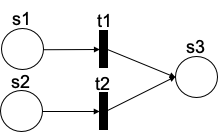
\includegraphics[width=.8\linewidth]{src/pic/OR.png}
  \captionof{figure}{OR-relationship}
  \label{fig:OR-relationship}
\end{minipage}%
\begin{minipage}{.5\textwidth}
  \centering
  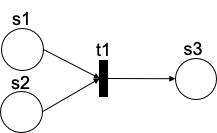
\includegraphics[width=.8\linewidth]{src/pic/AND.png}
  \captionof{figure}{AND-relationship}
  \label{fig:AND-relationship}
\end{minipage}
\end{figure}

\begin{figure}
\centering
\begin{minipage}{.5\textwidth}
  \centering
  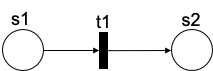
\includegraphics[width=.8\linewidth]{src/pic/SINGLE.png}
  \captionof{figure}{SINGLE-relationship}
  \label{fig:SINGLE-relationship}
\end{minipage}%
\begin{minipage}{.5\textwidth}
  \centering
  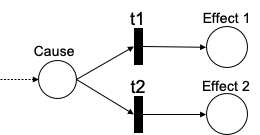
\includegraphics[width=.9\linewidth]{src/pic/ALTERNATE.png}
  \captionof{figure}{ALTERNATE-relationship}
  \label{fig:ALTERNATE-relationship}
\end{minipage}
\end{figure}

The most important of the four types of relationship is the ALTERNATE-relationship, because this is a non-determinism relationship, which means the place has more than one successor transition. In our algorithm, we focus on finding the ALTERNATE-relationship in the all Petri net to determine the causes and effects in the cause-effect-net.




